% --------------------------------------------------------------
% This is all preamble stuff that you don't have to worry about.
% Head down to where it says "Start here"
% --------------------------------------------------------------
 
\documentclass[12pt]{article}\usepackage[]{graphicx}\usepackage[]{color}
%% maxwidth is the original width if it is less than linewidth
%% otherwise use linewidth (to make sure the graphics do not exceed the margin)
\makeatletter
\def\maxwidth{ %
  \ifdim\Gin@nat@width>\linewidth
    \linewidth
  \else
    \Gin@nat@width
  \fi
}
\makeatother

\definecolor{fgcolor}{rgb}{0.345, 0.345, 0.345}
\newcommand{\hlnum}[1]{\textcolor[rgb]{0.686,0.059,0.569}{#1}}%
\newcommand{\hlstr}[1]{\textcolor[rgb]{0.192,0.494,0.8}{#1}}%
\newcommand{\hlcom}[1]{\textcolor[rgb]{0.678,0.584,0.686}{\textit{#1}}}%
\newcommand{\hlopt}[1]{\textcolor[rgb]{0,0,0}{#1}}%
\newcommand{\hlstd}[1]{\textcolor[rgb]{0.345,0.345,0.345}{#1}}%
\newcommand{\hlkwa}[1]{\textcolor[rgb]{0.161,0.373,0.58}{\textbf{#1}}}%
\newcommand{\hlkwb}[1]{\textcolor[rgb]{0.69,0.353,0.396}{#1}}%
\newcommand{\hlkwc}[1]{\textcolor[rgb]{0.333,0.667,0.333}{#1}}%
\newcommand{\hlkwd}[1]{\textcolor[rgb]{0.737,0.353,0.396}{\textbf{#1}}}%

\usepackage{framed}
\makeatletter
\newenvironment{kframe}{%
 \def\at@end@of@kframe{}%
 \ifinner\ifhmode%
  \def\at@end@of@kframe{\end{minipage}}%
  \begin{minipage}{\columnwidth}%
 \fi\fi%
 \def\FrameCommand##1{\hskip\@totalleftmargin \hskip-\fboxsep
 \colorbox{shadecolor}{##1}\hskip-\fboxsep
     % There is no \\@totalrightmargin, so:
     \hskip-\linewidth \hskip-\@totalleftmargin \hskip\columnwidth}%
 \MakeFramed {\advance\hsize-\width
   \@totalleftmargin\z@ \linewidth\hsize
   \@setminipage}}%
 {\par\unskip\endMakeFramed%
 \at@end@of@kframe}
\makeatother

\definecolor{shadecolor}{rgb}{.97, .97, .97}
\definecolor{messagecolor}{rgb}{0, 0, 0}
\definecolor{warningcolor}{rgb}{1, 0, 1}
\definecolor{errorcolor}{rgb}{1, 0, 0}
\newenvironment{knitrout}{}{} % an empty environment to be redefined in TeX

\usepackage{alltt}
 
\usepackage[margin=1in]{geometry} 
\usepackage{amsmath,amsthm,amssymb}
 \usepackage{amsfonts}
\newcommand{\N}{\mathbb{N}}
\newcommand{\Z}{\mathbb{Z}}
 
\newenvironment{theorem}[2][Theorem]{\begin{trivlist}
\item[\hskip \labelsep {\bfseries #1}\hskip \labelsep {\bfseries #2.}]}{\end{trivlist}}
\newenvironment{lemma}[2][Lemma]{\begin{trivlist}
\item[\hskip \labelsep {\bfseries #1}\hskip \labelsep {\bfseries #2.}]}{\end{trivlist}}
\newenvironment{exercise}[2][Exercise]{\begin{trivlist}
\item[\hskip \labelsep {\bfseries #1}\hskip \labelsep {\bfseries #2.}]}{\end{trivlist}}
\newenvironment{problem}[2][Problem]{\begin{trivlist}
\item[\hskip \labelsep {\bfseries #1}\hskip \labelsep {\bfseries #2.}]}{\end{trivlist}}
\newenvironment{question}[2][Question]{\begin{trivlist}
\item[\hskip \labelsep {\bfseries #1}\hskip \labelsep {\bfseries #2.}]}{\end{trivlist}}
\newenvironment{corollary}[2][Corollary]{\begin{trivlist}
\item[\hskip \labelsep {\bfseries #1}\hskip \labelsep {\bfseries #2.}]}{\end{trivlist}}
\newenvironment{BaseCase}[2][Base Case]{\begin{trivlist}
\item[\hskip \labelsep {\bfseries #1}\hskip \labelsep {\bfseries #2.}]}{\end{trivlist}}
\newenvironment{Answer}[2][Answer]{\begin{trivlist}
\item[\hskip \labelsep {\bfseries #1}\hskip \labelsep {\bfseries #2.}]}{\end{trivlist}}
\newenvironment{Sketch}[2][Sketch]{\begin{trivlist}
\item[\hskip \labelsep {\bfseries #1}\hskip \labelsep {\bfseries #2.}]}{\end{trivlist}}
\IfFileExists{upquote.sty}{\usepackage{upquote}}{}
\begin{document}
 
% --------------------------------------------------------------
%                         Start here
% --------------------------------------------------------------
 
\title{Homework 1}%replace X with the appropriate number
\author{Steve Bronder\\ %replace with your name
Statistical Inference} %if necessary, replace with your course title
 
\maketitle
 
\begin{exercise}{1}Find a dataset and evaluate whether Punxsutawney Phil can accurately predict six more weeks of winter
\end{exercise}

\section*{Answer}
 To evaluate whether Punxsutawney Phil can accurately predict six more weeks of winter we have to define a criteria for evaluation. Our criteria will be whether or not Phil accurately predicted a greater than average number of days with temperature below 32 degrees for the months of February and March of each year. If Phil predicts a long winter for a year we will give him 1 point out of a possible 65 points. Phil is limited to 65 points because our data ranges from 1950 to 2014 $(T=65)$. We gather data from the National Climate Data Center\footnote{http://www.ncdc.noaa.gov/cdo-web/datatools/findstation} for the county Punxsutawney Phil is located in, Jefferson County, PA. To find whether Phil saw his shadow we gather data from stormfax\footnote{http://www.stormfax.com/ghogday.htm} on whether or not he saw his shadow for our target years. \\

 Our data set is comprised of three variables, The year, the number of days it is below 32 degrees in the months of February and March, and whether or not Phil saw his shadow for a given year. Lets have a look at our data.
 
\begin{knitrout}
\definecolor{shadecolor}{rgb}{0.969, 0.969, 0.969}\color{fgcolor}\begin{kframe}
\begin{alltt}
\hlstd{ghog.data}\hlkwb{<-}\hlkwd{read.csv}\hlstd{(}\hlstr{"./ghog_clean.csv"}\hlstd{,}\hlkwc{header}\hlstd{=}\hlnum{TRUE}\hlstd{)}

\hlkwd{str}\hlstd{(ghog.data)}
\end{alltt}
\begin{verbatim}
## 'data.frame':	65 obs. of  3 variables:
##  $ Year    : int  1950 1951 1952 1953 1954 1955 1956 1957 1958 1959 ...
##  $ Snowfall: num  15 13 5 13 15 13 8 13 19 10 ...
##  $ ghog    : Factor w/ 2 levels "NOShadow","Shadow": 1 2 2 2 2 2 2 2 2 2 ...
\end{verbatim}
\begin{alltt}
\hlkwd{summary}\hlstd{(ghog.data[,}\hlnum{2}\hlopt{:}\hlnum{3}\hlstd{])}
\end{alltt}
\begin{verbatim}
##     Snowfall          ghog   
##  Min.   : 5.0   NOShadow:12  
##  1st Qu.:15.0   Shadow  :53  
##  Median :18.0                
##  Mean   :19.1                
##  3rd Qu.:25.0                
##  Max.   :31.0
\end{verbatim}
\end{kframe}
\end{knitrout}
 
 Notice that we do not have very many years Phil does not see his shadow (No six weeks of winter). Next we will create a variable for whether the amount of days it was below 32 degrees was greater than the average amount of days for a given year, whether Phil predicted a Long Winter, and whether his prediction was correct
 
\begin{knitrout}
\definecolor{shadecolor}{rgb}{0.969, 0.969, 0.969}\color{fgcolor}\begin{kframe}
\begin{alltt}
 \hlstd{ghog.data}\hlopt{$}\hlstd{gr.snowfall} \hlkwb{<-} \hlkwd{ifelse}\hlstd{(ghog.data}\hlopt{$}\hlstd{Snowfall}\hlopt{<}\hlkwd{mean}\hlstd{(ghog.data}\hlopt{$}\hlstd{Snowfall),}
                               \hlstr{"Long Winter"}\hlstd{,}\hlstr{"Short Winter"}\hlstd{)}
 \hlstd{ghog.data}\hlopt{$}\hlstd{gr.snowfall} \hlkwb{<-} \hlkwd{as.factor}\hlstd{(ghog.data}\hlopt{$}\hlstd{gr.snowfall)}

\hlstd{ghog.data}\hlopt{$}\hlstd{gr.ghog.predict} \hlkwb{<-} \hlkwd{ifelse}\hlstd{(ghog.data}\hlopt{$}\hlstd{ghog}\hlopt{==}\hlstr{"Shadow"}\hlstd{,}
                                  \hlstr{"Long Winter"}\hlstd{,}\hlstr{"Short Winter"}\hlstd{)}
\hlstd{ghog.data}\hlopt{$}\hlstd{gr.ghog.predict} \hlkwb{<-} \hlkwd{as.factor}\hlstd{(ghog.data}\hlopt{$}\hlstd{gr.ghog.predict)}

\hlstd{ghog.data}\hlopt{$}\hlstd{ghog.correct} \hlkwb{<-} \hlkwd{ifelse}\hlstd{(ghog.data}\hlopt{$}\hlstd{gr.ghog.predict}\hlopt{==}\hlstd{ghog.data}\hlopt{$}\hlstd{gr.snowfall,}
                               \hlstr{"Correct"}\hlstd{,}\hlstr{"Wrong"}\hlstd{)}
\hlstd{ghog.data}\hlopt{$}\hlstd{ghog.correct} \hlkwb{<-} \hlkwd{as.factor}\hlstd{(ghog.data}\hlopt{$}\hlstd{ghog.correct)}
\end{alltt}
\end{kframe}
\end{knitrout}
 
Now that we have created our variables lets generate a bar graph in ggplot2 that lets us examine the data further

\begin{knitrout}
\definecolor{shadecolor}{rgb}{0.969, 0.969, 0.969}\color{fgcolor}\begin{kframe}
\begin{alltt}
 \hlkwd{library}\hlstd{(ggplot2)}

\hlstd{ghog.graph} \hlkwb{<-} \hlkwd{ggplot}\hlstd{(ghog.data,} \hlkwd{aes}\hlstd{(ghog.correct,}\hlkwc{fill}\hlstd{=ghog))} \hlopt{+} \hlkwd{geom_bar}\hlstd{(}\hlkwc{width}\hlstd{=}\hlnum{.3}\hlstd{)} \hlopt{+}
   \hlkwd{theme_bw}\hlstd{()} \hlopt{+} \hlkwd{scale_fill_grey}\hlstd{(}\hlkwc{end}\hlstd{=}\hlnum{.8}\hlstd{)}

\hlstd{ghog.graph}
\end{alltt}
\end{kframe}
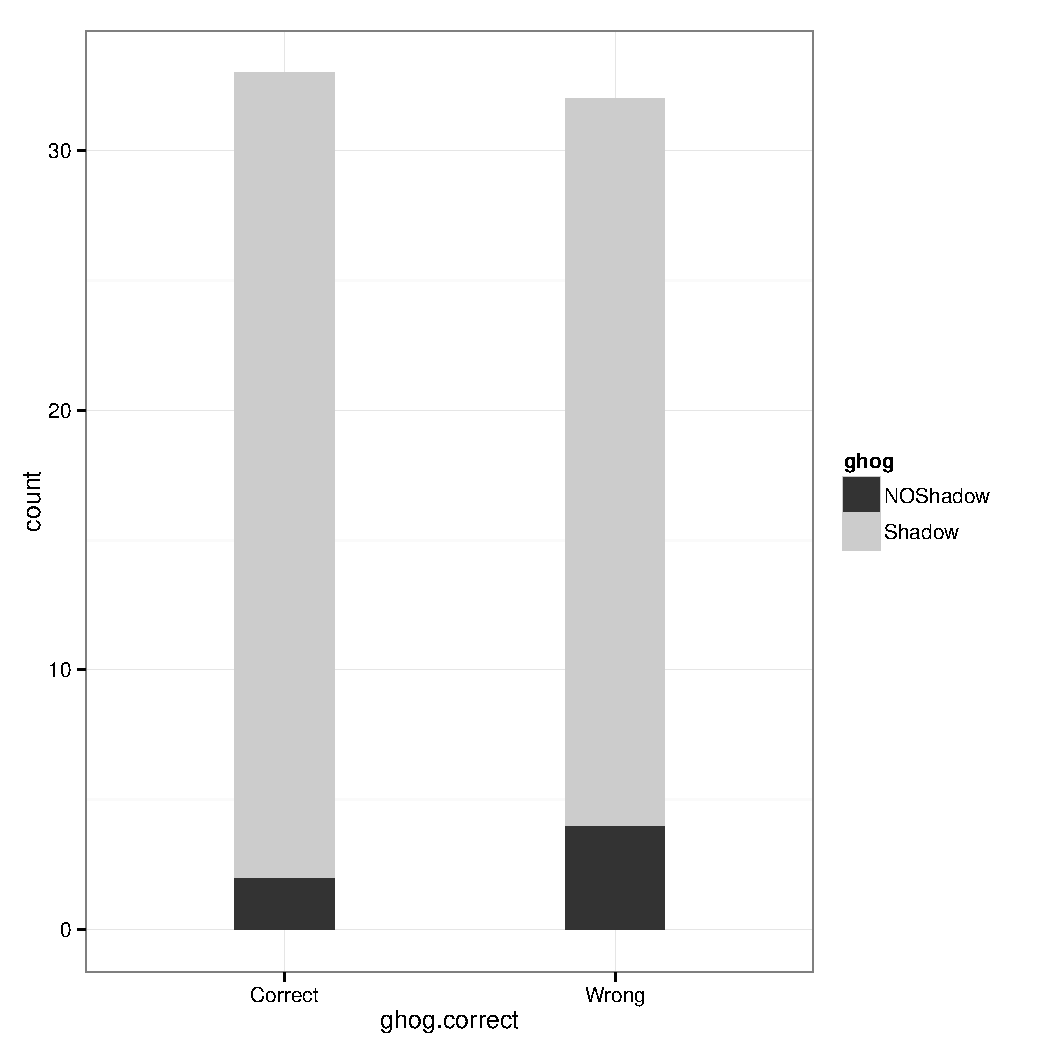
\includegraphics[width=\maxwidth]{figure/bargraph} 

\end{knitrout}

From this graph and table we can see he is correct 33 times and incorrect 32 times. Most of his errors are due to lacking short winter predictions. In fact, these prediction values are so close you could infer that Phil is probably as good at predicting the weather as the flip of a coin. This analysis find that  Punxsutawney Phil is wrong about fourty nine percent of the time. This is deemed a low score and so we conclude that Phil is a bad predictor of longer winters.

\newpage
% latex table generated in R 3.1.1 by xtable 1.7-4 package
% Tue Oct 21 18:35:45 2014
\begin{table}[ht]
\centering
\begin{tabular}{rlll}
  \hline
 &       gr.snowfall &     gr.ghog.predict &  ghog.correct \\ 
  \hline
1 & Long Winter :35   & Long Winter :53   & Correct:31   \\ 
  2 & Short Winter:30   & Short Winter:12   & Wrong  :34   \\ 
   \hline
\end{tabular}
\caption{Values for Number of Snowfalls, Groundhog Predictions, and Correct Groundhog Predictions} 
\end{table}
% latex table generated in R 3.1.1 by xtable 1.7-4 package
% Tue Oct 21 18:35:46 2014
\begin{table}[ht]
\centering
\begin{tabular}{rll}
  \hline
 & Prediction & Accuracy \\ 
  \hline
1 & Correct & 0.477 \\ 
  2 & Incorrect & 0.523 \\ 
   \hline
\end{tabular}
\caption{Percent of Correct and Incorrect Predictions} 
\end{table}



 
 
% --------------------------------------------------------------
%     You don't have to mess with anything below this line.
% --------------------------------------------------------------
 
\end{document}
